\chapter{Recomendaci\'on de configuraciones gr\'aficas basada en ML sobre grafos}\label{chapter:ml-on-graphs}

Los grafos son estructuras utilizadas extensivamente en la Ciencia de la Computaci\'on y otras
ramas de la ciencia debido a su capacidad de modelar escenarios donde se establecen relaciones entre un conjunto de objetos. 
Fen\'omenos
tan distintos como redes sociales, estructuras moleculares, redes de prote\'inas y
preferencias de usuarios pueden ser modelados mediante grafos.

En la actualidad, los grafos desempe\~nan un rol fundamental en el
aprendizaje de m\'aquinas. Se han dise\~nado muchos sistemas para hacer predicciones o descubrir patrones dentro
de datos representados con grafos. Por ejemplo, recomendar amigos en
redes sociales, clasificar el rol de las prote\'inas de acuerdo a sus interacciones
o predecir la ocurrencia de enlaces moleculares \cite{hamilton2017representation}.

En este cap\'itulo se presenta un marco de trabajo para modelar
el problema de recomendaci\'on de visualizaciones como un problema
de aprendizaje de m\'aquinas sobre grafos. En la secci\'on \ref{section:theoretical-framework}
se presenta el marco te\'orico necesario para la comprensi\'on del
resto del cap\'itulo y en la secci\'on \ref{section:graph-framework} se proponen
diferentes formas de modelaci\'on del problema. 


\section{Marco te\'orico-conceptual}\label{section:theoretical-framework}

En esta secci\'on se definen los conceptos principales de la teor\'ia de grafos
y se presentan las nociones b\'asicas del campo de aprendizaje de m\'aquinas
sobre grafos necesarias para el correcto entendimiento del marco de trabajo propuesto.

\subsection{Teor\'ia de grafos}

La teor\'ia de grafos se centra en el estudio de un modelo
matem\'atico propuesto por el matem\'atico Leonhard Euler en el
a\~no 1736 denominado grafo \cite{estrada2012structure}.

\begin{definition}
    Un \textbf{grafo} es un par formado por dos conjuntos $G = (V,E)$, 
    donde \\ $v \in V$ representa un v\'ertice (o nodo) del grafo y $E$ es un conjunto
    de pares no ordenados de elementos de $V$ a los cuales se les llama aristas. $G$ est\'a asociado con una funci\'on de tipado de v\'ertices $f_v: V \to \mathcal{T}^v$ y 
    una funci\'on de tipado de aristas $f_e : E \to \mathcal{T}^e$.  
\end{definition}

\begin{definition}
    Un grafo $G$ es \textbf{dirigido} si la existencia de la arista $\{v_i, v_j\} \in E$ no
    necesariamente implica la existencia de la arista sim\'etrica $\{v_j, v_i\} \in E$.
\end{definition}

\begin{definition}
    Un \textbf{grafo heterog\'eneo} $G_{hete}$ es un grafo tal 
    que $|\mathcal{T}^v| > 1 \vee |\mathcal{T}^e| > 1$. Existen v\'ertices y/o aristas
    de distinto tipo.
\end{definition}

\begin{definition}
    Un \textbf{grafo atributado} $G = (V,E,A,I)$ es una tupla de cuatro
    elementos, donde $V$ es un conjunto
    de v\'ertices, $E$ es un conjunto de aristas, $A$ es un
    conjunto de atributos e $I : V \cup E \to 2^A$ es una
    funci\'on que asigna conjuntos de atributos a los v\'ertices
    y aristas del grafo.
\end{definition}

\begin{definition}
    Un \textbf{grafo de conocimientos} $G_{know} = (V,E)$ es un grafo cuyos v\'ertices
    se consideran \textbf{entidades} y sus aristas son triplas de la forma $<h,r,t>$,
    donde $h, t \in V$ y $r$ representa el tipo de \textbf{relaci\'on} que se establece entre
    ambas entidades. 
\end{definition}



Los grafos pueden ser representados computacionalmente de distintas formas, las formas
m\'as utilizadas son la matriz de adyacencia y las listas de adyacencia.


\begin{definition}
    Dado un grafo $G = (V,E)$ la matriz de adyacencia de $G$ es una matriz
    $M^{|V|\times|V|}$ tal que:
    
    $$
            M_{ij} =
        \left\{
            \begin{array}{ll}
                1  & \mbox{if } \{v_i, v_j\} \in E \\
                0 & \mbox{if } e.o.c
            \end{array}
        \right.
    $$

\end{definition}


\begin{definition}
    Sea un grafo $G = (V,E)$ la lista de adyacencia de un v\'ertice $v \in V$ es el conjunto
    $\{ u \in V : \{v,u\} \in E \}$.
\end{definition}

Estas formas de representaci\'on de grafos han mostrado problemas de eficiencia
para la implementaci\'on de m\'etodos de an\'alisis de grafos, teniendo un
alto costo computacional y espacial. Por tanto, una de las principales l\'ineas de
investigaci\'on dentro de esta teor\'ia se dedica a la investigaci\'on de representaciones eficientes de grafos,
en el marco de esta l\'inea se define el problema de \textit{graph embedding} el cual se enfoca en representar
grafos mediante vectores.

\begin{definition}
    El \textbf{problema de graph embedding} consiste en, dado un grafo
    $G = (V,E)$ y un entero $k$, tal que $k \ll |V|$, representar el
    grafo $G$ en un espacio $k$-dimensional en el cual se deben de preservar
    las propiedades de dicho grafo. Si $G$ es un grafo de conocimientos este problema
    se denomina \textit{knowledge graph embedding} (KGE).
\end{definition}

\subsection{Aprendizaje de m\'aquinas sobre grafos}
Los problemas de aprendizaje de m\'aquinas sobre grafos suelen ser 
clasificados en cuatro tipo de problemas:

\begin{itemize}
    \item \textbf{Clasificaci\'on de v\'ertices: } El objetivo de este problema es, dado un grafo $G = (V,E)$,
    predecir las etiquetas $l_u$ (de tipo, categor\'ia o atributo) asociadas
    a los v\'ertices $u \in V$, utilizando las etiquetas de un conjunto de nodos de entrenamiento $V_{train} \subset V$.
    \item \textbf{Predicci\'on de aristas: } El objetivo de este problema es, dado un conjunto de
    v\'ertices $V$ y un conjunto incompleto de aristas $E_{train} \subset E$, inferir el conjunto
    de aristas faltantes $ E \setminus E_{train}$.
    \item \textbf{Detecci\'on de comunidades: } El problema de detecci\'on de comunidades es un problema de agrupamiento
    sobre los v\'ertices de un grafo $G$. Tiene como objetivo
    agrupar el conjunto de v\'ertices de forma tal que los v\'ertices pertenecientes
    a un mismo grupo tengan mayor similitud entre s\'i que con v\'ertices de otros grupos.
    \item \textbf{Clasificaci\'on, regresi\'on y agrupamiento de grafos: } La clasificaci\'on y regresi\'on de grafos son problemas
    an\'alogos a los problemas tradicionales de aprendizaje de m\'aquina supervisado donde se tienen como entrada un conjunto de
    datos de entrada $X$ (en este caso grafos), un conjunto de datos de salida $Y$ y se debe aproximar la funci\'on $h(X) = Y$. Igualmente,
    el problema de agrupamiento de grafos es an\'alogo al problema de aprendizaje no supervisado tradicional. 
\end{itemize}

Para resolver estos problemas, los primeros enfoques utilizaban estad\'isticas
descriptivas sobre grafos, funciones de kernel o medidas para caracterizar las
estructuras de vecindad de los v\'ertices. Sin embargo, estos enfoques son limitados ya que este tipo de medidas son inflexibles y no pueden ser adaptadas durante el proceso
de aprendizaje \cite{chakrabarti2006graph}. Un enfoque m\'as reciente
se basa en la soluci\'on del problema de \textit{graph embedding} mediante el aprendizaje
de funciones que permiten transformar v\'ertices, subgrafos o grafos enteros en
vectores del espacio $\mathbb{R}^K$. Este enfoque es
llamado \textit{Graph Representation Learning} (GRL) y ha permitido que
los grafos sean utilizados por m\'etodos tradicionales de aprendizaje de m\'aquinas \cite{hamilton2017representation}.


\section{Modelaci\'on de la recomendaci\'on de configuraciones visuales mediante grafos}\label{section:graph-framework}


El marco de trabajo propuesto en esta investigaci\'on consta de tres componentes que permiten definir y
comparar los elementos de un espacio de visualizaciones:

\begin{itemize}
    \item La representaci\'on matem\'atica de un lenguaje de visualizaci\'on de datos que permite 
    definir el espacio de b\'usqueda.
    \item La definici\'on de un conjunto de tareas de aprendizaje de m\'aquinas sobre grafos,
    cuyos resultados caracterizan los elementos del espacio de b\'usqueda.
    \item Una funci\'on que, utilizando las propiedades calculadas, le asigna una puntuaci\'on a
    cada elemento del espacio de b\'usqueda.
\end{itemize}

Una vez obtenidas las puntuaciones de los elementos del espacio de b\'usqueda las recomendaciones se realizan mediante el c\'omputo de las $k$ visualizaciones de mayor puntuaci\'on.

\subsection{Espacio de visualizaciones}\label{subsection:vis-space}

Siendo este trabajo un primer paso en este enfoque, se decidi\'o limitar su alcance
a las formas gr\'aficas tradicionales como gr\'aficos de barras, l\'ineas, entre otros. Estas formas
gr\'aficas est\'an dise\~nadas para la representaci\'on de datos estructurados, el modelo de 
datos usualmente empleado para representar conjuntos de datos estructurados es el modelo relacional \cite{codd1970relational}.
La representaci\'on de conjuntos de datos en este marco de trabajo est\'a basada en dicho modelo, permitiendo su
desarrollo sobre sistemas de bases de datos relacionales o sistemas de recomendaci\'on de visualizaciones que representen
la informaci\'on de forma relacional. Por tanto, un conjunto de datos es una \textit{relaci\'on} $R$, con atributos $A_1,A_2,...,A_n$, la cual puede representarse visualmente
como una tabla de filas y columnas.

Para poder generar una visualizaci\'on de $R$ es necesario
seleccionar las opciones gr\'aficas que codifican visualmente
cada uno de sus atributos. Este proceso se realiza de forma computacional mediante
la utilizaci\'on de lenguajes de visualizaci\'on para asociar los atributos a las distintas opciones.
Por este motivo se decidi\'o modelar la codificaci\'on visual de un conjunto de datos como 
una selecci\'on de opciones de configuraci\'on
gr\'afica en un lenguaje de visualizaci\'on abstracto.

\begin{definition}[Lenguaje de Visualizaci\'on de Datos]
    Un lenguaje de visualizaci\'on de datos $\mathcal{L}$ es un
    conjunto de elementos $C_i \in \mathcal{L}$, los cuales son una
    abstracci\'on de las configuraciones gr\'aficas permitidas dentro
    del lenguaje. Cada elemento $C_i$ es un conjunto de elementos
    $\{ c_{i1}, c_{i2},..., c_{i|C_i|}\}$, los cuales representan las
    posibles opciones de la configuraci\'on.
\end{definition}

Un ejemplo de la especificaci\'on de un lenguaje mediante la definici\'on anterior
ser\'ia $\mathcal{L} = \{ \texttt{Eje} = \{ \texttt{x}, \texttt{y} \}, 
\texttt{Marca} = \{ \texttt{l\'inea}, \texttt{punto}, \texttt{barra} \} \}$. 
Utilizando
este lenguaje un atributo puede ser codificado de seis formas distintas:
(\texttt{x}, \texttt{l\'inea}), (\texttt{x}, \texttt{punto}), \\(\texttt{x}, \texttt{barra}), (\texttt{y}, \texttt{l\'inea}),
(\texttt{y}, \texttt{punto}) y (\texttt{y}, \texttt{barra}), lo que da pie a la siguiente definici\'on:

\begin{definition}[Codificaci\'on visual]
    Sea un lenguaje de visualizaci\'on \\ $\mathcal{L} = \{ C_1, C_2, ..., C_n \}$,
    una codificaci\'on visual especificada en $\mathcal{L}$ es una tupla\\ $(c_1,c_2,...,c_n) \in C_1 \times C_2 \times ... \times C_n$.
    Se denota por $\mathbb{C}(\mathcal{L})$ al conjunto de todas las posibles codificaciones visuales
    que pueden ser especificadas en $\mathcal{L}$.
\end{definition}

% TODO: ta raro
La construcci\'on de una visualizaci\'on se realiza mediante
la selecci\'on de la codificaci\'on visual de cada uno de los atributos
del conjunto de datos. Se asume que el proceso de selecci\'on de la codificaci\'on visual de un
atributo es agn\'ostico a las codificaciones escogidas
para el resto de atributos del conjunto de datos. Por tanto,
todo atributo tiene  $|\mathbb{C}(\mathcal{L})|$ codificaciones
visuales posibles en el momento de seleccionar su codificaci\'on gr\'afica.

\begin{definition}[Espacio de visualizaciones]
    Sean $R$ un conjunto de datos de $n$ atributos y $\mathcal{L}$ un lenguaje de visualizaci\'on, el espacio
    de posibles visualizaciones de $R$ codificadas en $\mathcal{L}$ es $\mathbb{C}(\mathcal{L})^n$.
    
\end{definition}

\subsection{Caracterizaci\'on de conjuntos de datos}



En la actualidad, el an\'alisis de datos es aplicado a numerosas
ramas del conocimiento humano por lo
que los dominios de diferentes conjuntos de datos pueden ser muy heterog\'eneos.
Incluso, dentro de un mismo conjunto de datos los dominios pueden ser de
diferentes tipos (valores reales, cadenas, booleanos, etc...) y magnitudes.

Tomando en cuenta este problema, se decidi\'o caracterizar los conjuntos de datos
mediante la transformaci\'on de sus atributos a un espacio com\'un de dimensi\'on $K$.

\begin{definition}
    Se denota por $\mathcal{F}$ una familia de $K$ funciones que permiten transformar
    una atributo $A$ de dominio arbitrario (y perteneciente a una relaci\'on
    arbitraria) a un dominio $D$ de elementos at\'omicos.
    La representaci\'on de una funci\'on de esta familia ser\'ia
    $$
        f : \mathbb{A} \to \mathbb{D}
    $$
    donde $\mathbb{A}$ es el universo de atributos y $\mathbb{D}$ es el conjunto de posibles dominios.
\end{definition}

Esto permite representar a un atributo $A$ como un vector de $K$ dimensiones \\$ <f_1(A), f_2(A), ..., f_K(A)>$. Denotando dicho vector
por $\mathcal{F}(A)$ se puede extender este enfoque para un conjuntos de datos $S$ utilizando un conjunto de vectores \\
$\{ \mathcal{F}(A_1), \mathcal{F}(A_2), ..., \mathcal{F}(A_n)\}$.


\subsection{Tareas de aprendizaje de m\'aquinas}

El enfoque general para la resoluci\'on del problema es simular la
construcci\'on de un gr\'afico en un lenguaje de visualizaci\'on. Este proceso
consta de dos pasos:

\begin{enumerate}
    \item Seleccionar un atributo del conjunto de datos
    \item Seleccionar secuencialmente las opciones deseadas en la configuraci\'on gr\'afica de la visualizaci\'on: \begin{itemize}
        \item \tt Eje : x, y
        \item \tt Marca : barra, l\'inea, punto
    \end{itemize}
\end{enumerate}

N\'otese que para generar el gr\'afico el usuario resuelve una serie de problemas de decisi\'on sobre las configuraciones gr\'aficas.
Por este motivo dado un lenguaje de visualizaci\'on $\mathcal{C}$ con configuraciones gr\'aficas $C_1, C_2, ..., C_n$
se define una tarea de aprendizaje de m\'aquinas por cada configuraci\'on $C_i$ cuyo resultado es interpretado para escoger las opciones.

% Es importante resaltar que se consideraron dos tipos de configuraciones gr\'aficas: las asociadas
% a los atributos (p.e. eje, color, marca) y las asociadas al conjunto de datos (p.e. utilizaci\'on de leyendas y cuadr\'iculas).

\subsubsection{Problema de clasificaci\'on de v\'ertices}

Para este problema se construye un grafo de conocimientos definiendo
los siguientes conjuntos de v\'ertices y aristas:

\begin{itemize}
    \item Conjunto de v\'ertices $V_A$: este conjunto representa los atributos del conjunto de datos.
    \item Conjunto de v\'ertices $V_F$: este conjunto representan los valores obtenidos al aplicar las 
    funciones de $\mathcal{F}$ sobre los atributos del conjunto de datos. 
    \item Conjunto de aristas $E_{AF}$: este conjunto representa la relaci\'on de caracterizaci\'on entre los valores 
    computados por las funciones de $\mathcal{F}$ y los atributos. Las aristas de este conjunto son triplas de la forma $<f_j(a_i), f_j, a_i>$,
    donde $a_i \in V_A, \;f_j \in \mathcal{F}$ y $f_j(a_i) \in V_F$.
\end{itemize}


Luego se define la tarea de aprendizaje de la siguiente forma:

    Sean un grafo $G = (V,E)$ con $V = V_A \cup V_F$ y $E = E_{AF}$, una configuraci\'on
gr\'afica $C$ y un conjunto $\mathcal{L}$ de etiquetas tal que existe una funci\'on biyectiva $f : \mathcal{L} \to C$.
Dado un conjunto de v\'ertices ${V_A}_l \subset V_A $ los cuales est\'an etiquetados el objetivo es aproximar la funci\'on
$h : V_A \to \mathcal{L}$ para inferir las
etiquetas para el conjunto $V_A \setminus {V_A}_l$ de v\'ertices no etiquetados. 


\begin{center}
    \begin{figure}[h!]
        \centering
        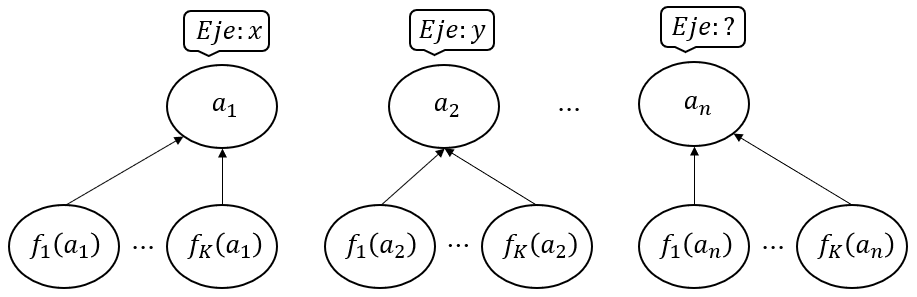
\includegraphics[width=130mm, height=60mm]{Graphics/graph_class_kg.png}
        \caption{Estructura de grafo propuesta para el problema de clasificaci\'on de v\'ertices}
        \label{fig: graph-struct}
    \end{figure}
\end{center}




\subsubsection{Problema de predicci\'on de aristas}

En este problema se modific\'o la estructura del grafo mostrada por la Figura \ref{fig: graph-struct}
a\~nadiendo el conjunto de v\'ertices $V_C$ el cual representa las posibles opciones de una configuraci\'on $C_i$ y
el conjunto de aristas $E_{AC}$ las cuales representan la utilizaci\'on de una opci\'on para codificar un atributo.\\\\

\begin{figure}[h!]
    \centering
    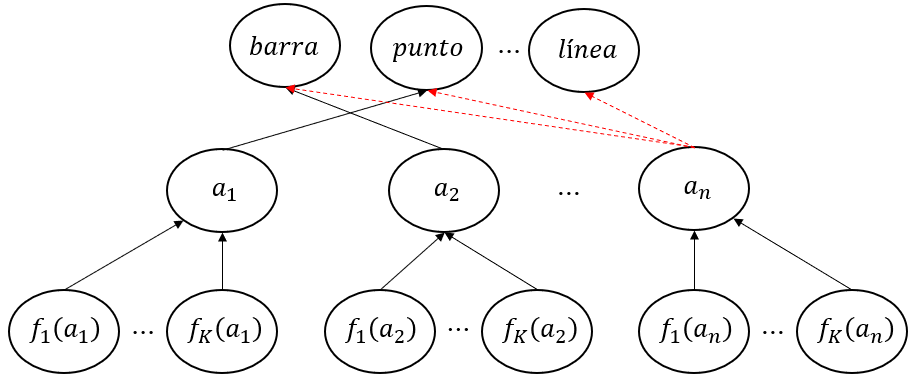
\includegraphics[width=130mm, height=65mm]{Graphics/link_pred_kg.png}
    \caption{Estructura de grafo propuesta para el problema de predicci\'on de aristas.}
    \label{fig: link-pred-graph}
\end{figure}

La tarea de aprendizaje es definida como:


    Sean un grafo $G = (V,E)$ con $V = V_A \cup V_F \cup V_C$ y $E = E_{AF} \cup E_{AC}$,
    una configuraci\'on gr\'afica $C$ y $E_{AC}^*$ el conjunto de todas las posibles aristas entre los conjuntos de v\'ertices $V_A$ y $V_C$.
    El objetivo es aproximar una funci\'on de probabilidad $p : E_{AC}^* \to [0,1]$ la cual indique la probabilidad de que una arista
    entre un elemento $V_A$ y un elemento de $V_C$ pertenezca al grafo.



% \subsection{Problema de clasificaci\'on de grafos}
% Conjunto de conjunto de datos $V_D$: este conjunto representa los conjuntos de datos.

% \textit{Pertenecer} $E_{AD}$: este conjunto de aristas representa la relaci\'on de pertenencia entre un atributo y un conjunto de datos.

% Sean $C$ una configuraci\'on gr\'afica, $\mathcal{L}$ un conjunto de etiquetas y
% una funci\'on biyectiva $f : \mathcal{L} \to C$. Dado un conjunto
% de grafos etiquetados $\{(G_1, l_1), (G_2, l_2),..., (G_n, l_n)\}$, $l_i \in \mathcal{L} : 1 \leq i \leq n$ 
% el objetivo es aproximar una funci\'on $h : \mathbb{G} \to \mathcal{L}$ donde
% $\mathbb{G}$ es el espacio de todos los posibles grafos.

\subsection{Funci\'on de puntuaci\'on}\label{subsection:score-func}

Partiendo de los elementos propuestos en las secciones anteriores se considera un conjunto
de datos $R$ con atributos $A_1, A_2, ..., A_n$ y un lenguaje de visualizaci\'on $\mathcal{L} = \{C_1,C_2,...,C_m\}$.
Por cada configuraci\'on $C_i$ se tiene un modelo $\mathcal{M}_i$, que evaluado en los atributos $A_1, A_2, ...,A_n$
devuelve como salida una matriz $P^{(i)}$ de dimensi\'on $n\times|C_i|$. El
valor $P^{(i)}_{jk}$ representa la probabilidad de que el $j$-\'esimo atributo sea codificado
utilizando la $k$-\'esima opci\'on de la configuraci\'on $C_i$.

Se define la funci\'on $\phi : \mathbb{A} \times \mathbb{C}(\mathcal{L}) \to \mathbb{R}$
como:
    $$
        \phi(A_j, (c_{k_1},c_{k_2},...,c_{k_{|\mathcal{L}|}} )) = \overset{|\mathcal{L}|}{\underset{i=1}{ \prod }}P^{(i)}_{jk_{i}}
    $$

Luego, dada una visualizaci\'on $\mathcal{V}$ especificada por las codificaciones $\mathcal{C}_1, \mathcal{C}_2, ..., \mathcal{C}_n$,
donde $\mathcal{C}_i$ es la codificaci\'on visual del atributo $A_i$, se calcula la puntuaci\'on de $\mathcal{V}$ como:

$$
           \overset{n}{\underset{i=1}{\prod}} \phi(A_i, \mathcal{C}_i)
$$


N\'otese que esta funci\'on penaliza gravemente aquellas visualizaciones
constru\'idas con opciones de poca probabilidad de ocurrencia.

En la literatura especializada existen diversos modelos de aprendizaje de m\'aquinas  para
la soluci\'on de tareas de clasificaci\'on \cite{aly2005survey} y predicci\'on de aristas \cite{lu2011link}.
Para definir la funci\'on de puntuaci\'on se asume que la salida de los modelos utilizados es una distribuci\'on
de probabilidades discreta. Una alternativa para utilizar modelos que no satisfacen
esta restricci\'on ser\'ia normalizar la salida del modelo utilizando la funci\'on \textit{softmax}.


\chapter{MLG4Vis}\label{chapter:proposal}

En la actualidad los analistas de datos realizan su trabajo
sobre conjuntos de datos de gran tama\~no y dimensi\'on por lo que
necesitan herramientas computacionales que apoyen y faciliten
el proceso de exploraci\'on de datos.

A continuaci\'on se describe un prototipo de sistema de recomendaci\'on de
configuraciones gr\'aficas con el objetivo de que pueda ser utilizado
por plataformas de an\'alisis de datos, sea dentro de un an\'alisis manual o 
automatizado. Esta propuesta de soluci\'on se fundamenta en los conceptos
y problemas presentados en el cap\'itulo \ref{chapter:ml-on-graphs}.

\section{Concepci\'on y dise\~no del sistema}

\begin{figure}[h!]
    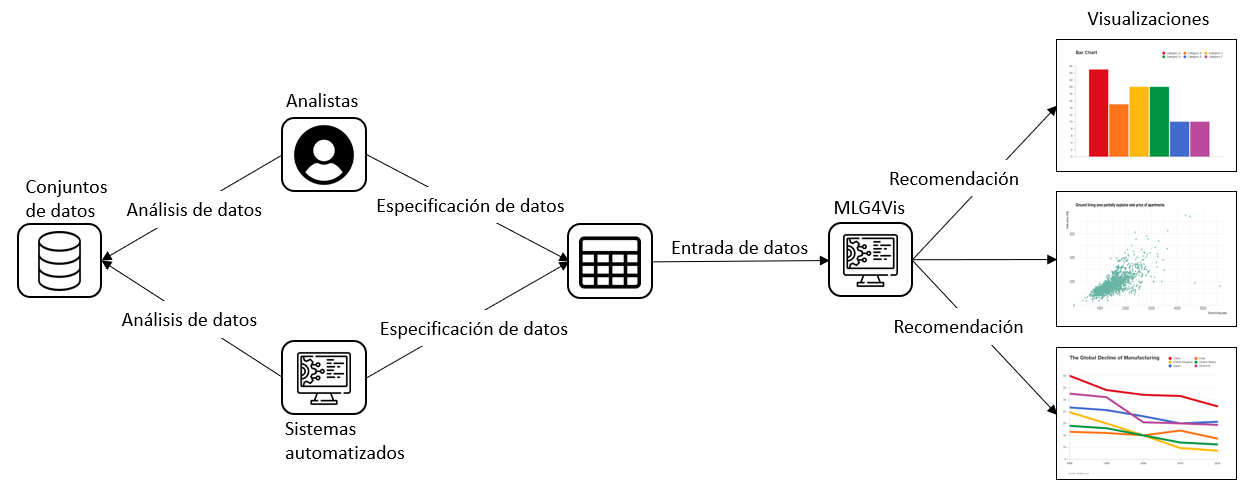
\includegraphics[width=\linewidth]{Graphics/mlg4vis.png}
    \caption{Utilizaci\'on de MLG4Vis en el an\'alisis de datos}
    \label{fig: mlg4vis}
\end{figure}


\textit{Machine Learning on Graphs For Visualization} (MLG4Vis) se concibe como un
sistema el cual pueda ser utilizado dentro de plataformas de an\'alisis de datos. Estas plataformas
deben permitir una especificaci\'on parcial de las visualizaciones, pudiendo el
usuario seleccionar la informaci\'on a ser visualizada u obtener esta mediante sistemas
automatizados como LETO (Figura \ref{fig: mlg4vis}).

MLG4Vis est\'a dividido en 4 m\'odulos interrelacionados que
constituyen la implementaci\'on del enfoque propuesto en el cap\'itulo \ref{chapter:ml-on-graphs}.
Cada m\'odulo
tiene una responsabilidad espec\'ifica mediante la definici\'on de datos
de entrada y salida que caracterizan la intercomunicaci\'on con el resto de los
m\'odulos.

\begin{figure}[h!]
    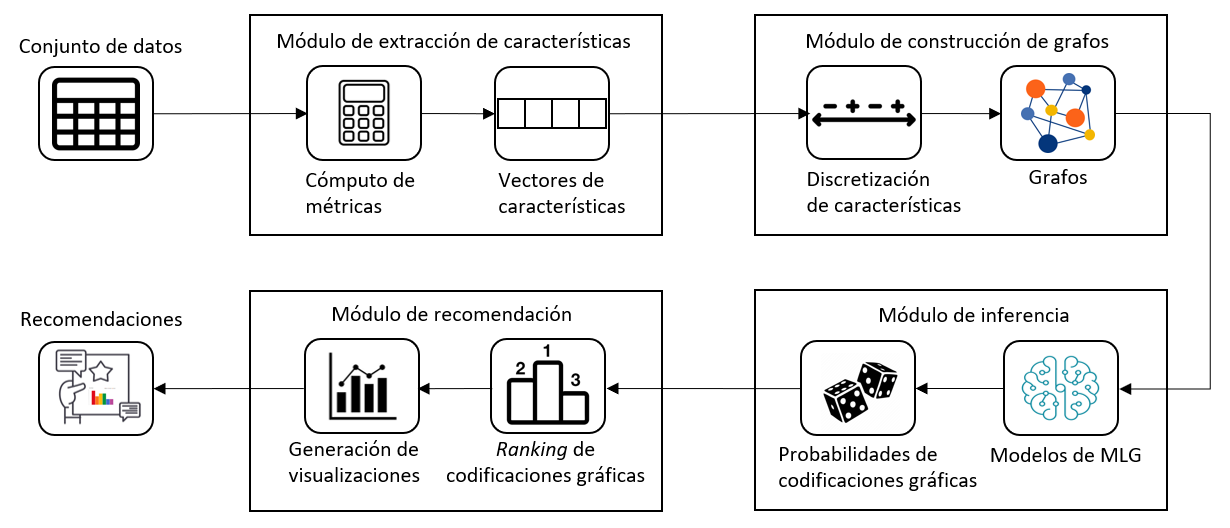
\includegraphics[width=\linewidth]{Graphics/mlg4vis-arch.png}
    \caption{Arquitectura de MLG4Vis}
    \label{fig: mlg4vis-arch}
\end{figure}

Como se puede apreciar en la Figura \ref{fig: mlg4vis-arch} los
4 m\'odulos est\'an dispuestos de forma secuencial modelando
la transformaci\'on de un conjunto de datos en recomendaciones.

\begin{itemize}
    \item La entrada del sistema la constituye un conjunto de datos estructurados.
    \item El \textbf{M\'odulo de extracci\'on de caracter\'isticas} computa una serie
    de m\'etricas que permiten describir el conjunto de datos como un conjunto de vectores de caracter\'isticas.
    \item El \textbf{M\'odulo de construcci\'on de grafos} realiza un proceso de discretizaci\'on
    sobre las caracter\'isticas continuas de los vectores y procede a construir los grafos propuestos
    en el cap\'itulo \ref{chapter:ml-on-graphs}.
    \item El \textbf{M\'odulo de inferencia} implementa los modelos
    que computan los vectores de probabilidades para las configuraciones gr\'aficas mediante la resoluci\'on
    de las tareas propuestas en el cap\'itulo \ref{chapter:ml-on-graphs}.
    \item El \textbf{M\'odulo de recomendaci\'on} se encarga de construir las visualizaciones
    utilizando las probabilidades computadas por los modelos de
    aprendizaje de m\'aquinas sobre grafos y realiza un \textit{ranking}
    de las visualizaciones.
    \item El \textit{ranking} de visualizaciones obtenido se retorna como salida del sistema en forma de
    recomendaciones.
\end{itemize}

En las secciones a continuaci\'on se expone de forma general el funcionamiento de los distintos m\'odulos
del sistema y las principales consideraciones tomadas durante su dise\~no.

\section{M\'odulo de extracci\'on de caracter\'isticas}

Este m\'odulo se encarga de transformar el conjunto de datos de entrada a un
espacio com\'un de vectores de $K$ dimensiones mediante el c\'omputo de m\'etricas. 

Antes de proceder a calcular las m\'etricas el conjunto de datos de entrada es preprocesado.
Primero, se realiza (de ser necesario) una inferencia del tipo de los atributos del conjunto de datos ya que existen
varios formatos de almacenamiento de datos (p.e. valores separados por comas) que no almacenan los metadatos
respectivos al dominio de los atributos. Luego se aborda un problema com\'un dentro del an\'alisis de datos que
es la existencia de datos faltantes \cite{schafer2002missing}. Este problema ha sido extensamente estudiado en la Estad\'istica 
debido a que puede comprometer la calidad de las mediciones estad\'isticas obtenidas. Para
resolver este problema se utilizaron t\'ecnicas de imputaci\'on de datos \cite{jadhav2019comparison}.

Terminado el preprocesamiento se procede a realizar el c\'alculo de una serie de medidas. La mayor\'ia
de estas medidas provienen del campo de la Estad\'istica y fueron seleccionadas de acuerdo a su robustez
ante la diferencia de magnitudes que pueden existir en los distintos conjuntos de datos.

\section{M\'odulo de construcci\'on de grafos}

Previo a la construcci\'on del grafo se realiza un proceso
de discretizaci\'on de las componentes de los vectores para reducir
la cantidad de v\'ertices del grafo que surgen como representaciones de valores en un dominio continuo.
Cada componente es discretizada mediante la creaci\'on de intervalos que particionan el
rango de valores que puede tomar. Para este proceso
se utiliz\'o el algoritmo MDLP \cite{fayyad1993multi}, el cual puede
inferir la cantidad de intervalos en que deben ser particionados los valores
bas\'andose en la distribuci\'on de los datos. 

Luego se procede a construir los grafos de acuerdo a las estructuras propuestas en el cap\'itulo \ref{chapter:ml-on-graphs}.
Es importante destacar que este m\'odulo construye dos tipos de grafos: un grafo de entrenamiento a partir de un corpus y
grafos de inferencia a partir de los conjuntos de datos de entrada. La diferencia entre estos dos tipos de grafos es la utilizaci\'on
del algoritmo MDLP, este solo se utiliza en la construcci\'on del grafo de entrenamiento ya
que los intervalos generados son reutilizados por los grafos de inferencia.
\section{M\'odulo de inferencia}

Una vez obtenidos los grafos de conocimientos que modelan los conjuntos de datos se procedi\'o
a dise\~nar modelos que resuelvan las tareas de aprendizaje de m\'aquinas propuestas en el cap\'itulo \ref{chapter:ml-on-graphs}.

Dentro del aprendizaje de m\'aquinas sobre grafos existen m\'ultiples modelos para solucionar las tareas propuestas 
[\cite*{hamilton2017representation}, \cite*{chami2022machine},  \cite*{cai2018comprehensive}, \cite*{nickel2015review}], por lo que a continuaci\'on se presentan
los criterios utilizados en la b\'usqueda de algoritmos para este escenario:

\begin{enumerate}
    \item El algoritmo debe poder utilizarse sobre grafos dirigidos, no atributados y heterog\'eneos con
    v\'ertices y aristas de distinto tipo.
    \item El algoritmo debe poder ser utilizado con datos no observados durante el entrenamiento, debido
    a que los analistas trabajan con nuevos conjuntos de datos de forma constante.
\end{enumerate}

Esta b\'usqueda no arroj\'o resultados
satisfactorios, por lo que se procedi\'o a investigar
c\'omo adaptar los algoritmos
que incumplen la segunda condici\'on para su uso en este problema. Estos modelos,
clasificados en la literatura como \textit{transductivos}, funcionan
como un diccionario que asocia cada elemento del grafo con su representaci\'on
vectorial \cite{cai2018comprehensive}. Debido a esto deben ser entrenados cada vez que un nuevo conjunto de datos
sea procesado por el sistema, lo cual provocar\'ia largos tiempos de espera para el usuario.

Para permitir la utilizaci\'on de los modelos transductivos se seleccion\'o la metaheur\'istica de \textit{universos paralelos}, esta
fue dise\~nada para obtener aproximaciones a problemas de enrutamiento de veh\'iculos \cite{bayat2014parallel} y ha sido
adaptada de forma satisfactoria para su uso en \textit{Graph Representation Learning} con el m\'etodo transductivo TransE \cite{tay2017non}.
% La adaptaci\'on de este m\'etodo a las necesidades del sistema
% se centra en la reducci\'on del tiempo de entrenamiento de los modelos
% transductivos 

% El objetivo de este m\'etodo es permitir la aplicaci\'on de t\'ecnicas transductivas
% de \textit{Graph Representation Learning} al problema de naturaleza inductiva de clasificar
% atributos no vistos durante el entrenamiento.

A continuaci\'on se discute el funcionamiento de este algoritmo y su adaptaci\'on al contexto de la
selecci\'on de configuraciones gr\'aficas.


\subsection{Inferencia mediante universos paralelos}

La metaheur\'istica de universos paralelos intenta reducir el tiempo de
entrenamiento necesario para construir un modelo al ser analizado
un nuevo conjunto de datos. Esto se realiza mediante el
entrenamiento de modelos de menor complejidad producidos sobre
un grafo de muestra mucho m\'as peque\~no que el original. Para
generar un decisi\'on se establece un m\'etodo de consenso 
entre los distintos modelos creados.


La base del funcionamiento de este algoritmo es la construcci\'on de
un conjunto de $N$ universos de \textit{embedding} $\Delta = \{\Delta_1, \Delta_2, ..., \Delta_N\}$
a partir de un grafo de entrenamiento $G_{train}$ y un grafo sobre el que realizar inferencia $G_{inf}$.
Estos grafos utilizan la misma estructura (Figuras \ref{fig: graph-struct}, \ref{fig: link-pred-graph}) y comparten el espacio discretizado
para representar los atributos, es decir, $V_F(G_{Train}) = V_F(G_{inf})$.

Cada universo $\Delta_i$ est\'a definido por dos elementos:
\begin{enumerate}
    \item Un grafo $G_i$ tal que $G_i \subset G_{train} \cup G_{inf}$ y $|G_i| \lll |G_{train} \cup G_{inf}|$.
    Para la construcci\'on de este grafo se definen tres par\'ametros $\alpha$, $\beta$ y $\gamma$ cuyos valores son aleatorios.
    Primero, se escoge aleatoriamente un conjunto de $\alpha$ funciones $\mathcal{F}_\alpha \subset \mathcal{F}$
    que define las caracter\'isticas de los atributos del universo. Las aristas de los
    grafos $G_{train}$ y $G_{inf}$ que no representan funciones de $\mathcal{F}_\alpha$ son descartadas. Luego se procede a construir
     dos subgrafos de $G_{train}$:
    \begin{itemize}
        \item Se selecciona, de forma aleatoria, un conjunto de $\beta$ v\'ertices de $V_A(G_{train})$
        que tengan al menos una caracter\'istica en com\'un con un v\'ertice de $G_{inf}$.
        El grafo $G_\beta$ es el grafo inducido sobre $G_{train}$ por los v\'ertices seleccionados.
        Con esto se intenta muestrear atributos similares a aquellos de los que se quiere predecir su configuraci\'on.
        \item El grafo $G_\gamma$ es el grafo inducido sobre $G_{train}$ por un conjunto de $\gamma$
        v\'ertices de $V_A(G_{train})$, muestreados uniformemente con respecto al valor de la configuraci\'on gr\'afica. Es decir,
        en este grafo cada posible valor de la configuraci\'on gr\'afica est\'a relacionado con la misma cantidad de atributos. Esto se realiza
        para disminuir sesgos en el universo como, por ejemplo, que una de las opciones gr\'afica no exista.
    \end{itemize}
    Finalmente, se construye el grafo $G_i = G_{inf} \cup G_\beta \cup G_\gamma$. 
    \item Un flujo\footnote[1]{Se refiere a la palabra \textit{pipeline} encontrada en la literatura} de \textit{embedding}
    compuesto por un algoritmo de \textit{embedding} $\mathcal{E}_i$ y un conjunto $\Theta_i$ de hiperpar\'ametros de $\mathcal{E}_i$.
    Estos son seleccionados de forma aleatoria y, una vez obtenidos, se entrena el algoritmo
    de \textit{embedding} sobre el grafo $G_i$ para obtener el modelo $\mathcal{M}_i(\mathcal{E}_i, \Theta_i, G_i)$.
\end{enumerate} 

Dado un conjunto $\Delta$ de universos se define un mecanismo de
consenso entre los modelos entrenados. Para seleccionar
la opci\'on de configuraci\'on visual de un atributo se
realiza una votaci\'on, donde cada modelo vota
por la opci\'on que considera m\'as probable. El resultado
de esta votaci\'on es almacenado en un vector que luego
es normalizado a una distribuci\'on de probabilidades utilizando
la funci\'on \textit{softmax}. La $i$-\'esima componente de
este vector es la probabilidad de que el atributo sea codificado
utilizando le $i$-\'esima opci\'on de la configuraci\'on gr\'afica.



\begin{algorithm}[H]
    \caption{Generaci\'on de universos paralelos}\label{alg:meta-pu}
    \KwData{Configuraci\'on gr\'afica $C$, conjunto de funciones $\mathcal{F}$, grafo de entrenamiento $G_{train}$, grafo de inferencia $G_{inf}$, n\'umero de universos paralelos $N$}
    \KwResult{Conjunto $\Delta$ de $N$ universos paralelos}

    $\Delta \gets$ inicializar conjunto vac\'io de universos paralelos\\
    \For{$i=1...N$}{
        $\alpha, \beta, \gamma \gets$ generar par\'ametros aleatorios\\
        $\mathcal{F}_\alpha \gets$ seleccionar $\alpha$ funciones de $\mathcal{F}$\\
        $G_{train} \gets G_{train} - \{<h,r,t> : r \notin \mathcal{F}_\alpha\}$\\
        $G_{inf} \gets G_{inf} - \{<h,r,t> : r \notin \mathcal{F}_\alpha\}$\\
        $V_\beta \gets$ seleccionar $\beta$ v\'ertices de $\{ v \in V(G_{train}) : \exists f \in \mathcal{F}_\alpha \, \exists u \in G_{inf}\, f(v) = f(u)\}$\\
        $G_\beta \gets$ generar subgrafo de $G_{train}$ inducido por $V_\beta$\\
        $V_\gamma \gets \emptyset$\\
        \For{$j=1...|C|$}{
            $V_{c_j} \gets$ seleccionar $\frac{\gamma}{|C|}$ v\'ertices de $\{ v \in V(G_{train}) : c_j \; \textnormal{es la opci\'on de configuraci\'on gr\'afica asociada a} \; v\}$\\
            $V_\gamma \gets V_\gamma \cup V_{c_j}$
        }
        $G_\gamma \gets$ generar subgrafo de $G_{train}$ inducido por $V_\gamma$\\
        $G_i \gets G_{inf} \cup G_\beta \cup G_\gamma$\\
        $\mathcal{E}_i, \Theta_i \gets$ generar algoritmo de \textit{embedding} e hiperpar\'ametros aleatorios\\
        $\mathcal{M}_i(\mathcal{E}_i, \Theta_i, G_i) \gets$ entrenar el algoritmo de \textit{embedding} en el grafo $G_i$\\
        $\Delta \gets$ a\~nadir el modelo $\mathcal{M}_i(\mathcal{E}_i, \Theta_i, G_i)$ al conjunto de universos
    }
    
\end{algorithm}

\subsection{Selecci\'on de algoritmos}

La metaheur\'istica presentada selecciona de 
forma aleatoria un algoritmo de KGE (\textit{knowledge graph embedding}) para
cada universo, por tanto, se hace necesario definir
un conjuntos de posibles algoritmos que puedan ser
utilizados. En esta investigaci\'on se seleccionaron
los algoritmos TransD \cite{ji-etal-2015-knowledge}, TransE \cite{bordes2013translating}, TransH \cite{wang2014knowledge} y TransR \cite{lin2015learning}.
Adem\'as, se
consideraron los siguientes tipos de hiperpar\'ametros:

\begin{itemize}
    \item Hiperpar\'ametros de representaci\'on: dimensi\'on del espacio de \textit{embedding}, definici\'on de norma utilizada en el espacio de vectores, etc.
    \item Hiperpar\'ametros de optimizaci\'on: optimizador utilizado, raz\'on de aprendizaje, etc.
    \item Hiperpar\'ametros de entrenamiento: estrategia de entrenamiento, cantidad de \'epocas, etc.
\end{itemize}

Es importante destacar que los algoritmos de
KGE seleccionados no implementan de forma natural la
clasificaci\'on de v\'ertices. Por lo cual, se debe de
entrenar un modelo de clasificaci\'on utilizando, como datos
de entrada, las representaciones vectoriales de los
v\'ertices generadas por el modelo KGE. Los modelos
de clasificaci\'on utilizados
deben soportar la existencia de m\'ultiples clases y
predecir la probabilidad de pertenencia de los elementos a cada una. De
acuerdo a estos criterios se escogi\'o el modelo K-Nearest Neighbors (KNN).


\section{M\'odulo de recomendaci\'on}
Este m\'odulo computa todas las posibles visualizaciones para el conjunto de
datos de acuerdo con los conceptos presentados en la secci\'on \ref{subsection:vis-space}.
Adem\'as, se establecen restricciones de integridad sobre las visualizaciones, por ejemplo,
cada eje de la visualizaci\'on debe tener asociado un atributo.

Utilizando las matrices de probabilidades obtenidas
de los modelos de aprendizaje de m\'aquinas sobre grafos, se calcula la puntuaci\'on de las visualizaciones
utilizando la funci\'on definida en la secci\'on \ref{subsection:score-func}. Las $k$ visualizaciones
de mayor puntuaci\'on son seleccionadas, y se procede a construir sus
gr\'aficos utilizando un lenguaje de visualizaci\'on de datos de alto nivel. Finalmente,
estas visualizaciones son presentadas al usuario en forma de recomendaciones.



